\chapter{Application to Quantum Information}
\label{ch:chapter3}
\ifpdf
    \graphicspath{{Chapter3/Chapter3Figs/PNG/}{Chapter3/Chapter3Figs/PDF/}{Chapter3/Chapter3Figs/}}
\else
    \graphicspath{{Chapter3/Chapter3Figs/EPS/}{Chapter3/Chapter3Figs/}}
\fi

Entanglement is the fundamental inseparability of quantum systems - seen as correlations that emerge in quantum theory and that cannot be described by classical physics. It has been described as ``the strangest and least understood facet of quantum theory''\cite{Rudolph} and this, in itself, provides a good motivation for the study of quantum entanglement. Furthermore, some future technologies such as quantum computers, quantum teleportation and ion clocks\cite{Rudolph} rely on the unique properties of entanglement. A method that can calculate measures of entanglement between qubits or systems of qubits could prove useful in the development of such technologies. 

Currently, there are no known scalable simulation methods\cite{Hastings2010} that are capable of calculating entanglement measures. Entanglement simulations rely on non-scalable algorithms such as density matrix renormalisation group (DMRG) or Lanczos. Other QMC methods do not provide access to the reduced density matrix. However, with DMQMC and the stochastic sampling of the full density matrix, it is possible to obtain the reduced density matrix.

This chapter begins by introducing the two main measures of entanglement (concurrence and Von-Neumann entropy) in quantum information theory. It moves on to discuss how estimators for such methods can be incorporated into the DMQMC algorithm. Finally, the estimator for concurrence is tested against some simple 1D antiferromagnetic Heisenberg rings in the presence and absence of an applied magnetic field.

\section{Reduced Density Matrix}

A major obstacle that prevents QMC simulations of entanglement measures in many-electron quantum systems is the difficulty of obtaining the reduced density matrix. In DMQMC, it is possible to obtain a reduced density matrix for a small subsystem (small enough so that it can be stored and manipulated in computer memory).

Consider two quantum systems $A$ and $B$ that are coupled to form a system $C$ (Fig.~\ref{fig:coupledSubsystems}) such that
\begin{equation}
\mathcal{H}_C = \mathcal{H}_A \otimes \mathcal{H}_B,
\label{eqn:coupledSubsystems}
\end{equation}
where $\mathcal{H}_A$, $\mathcal{H}_B$ and $\mathcal{H}_C$  denote the Hilbert spaces of systems $A$, $B$ and $C$. 
\begin{figure}[H]
\begin{center}
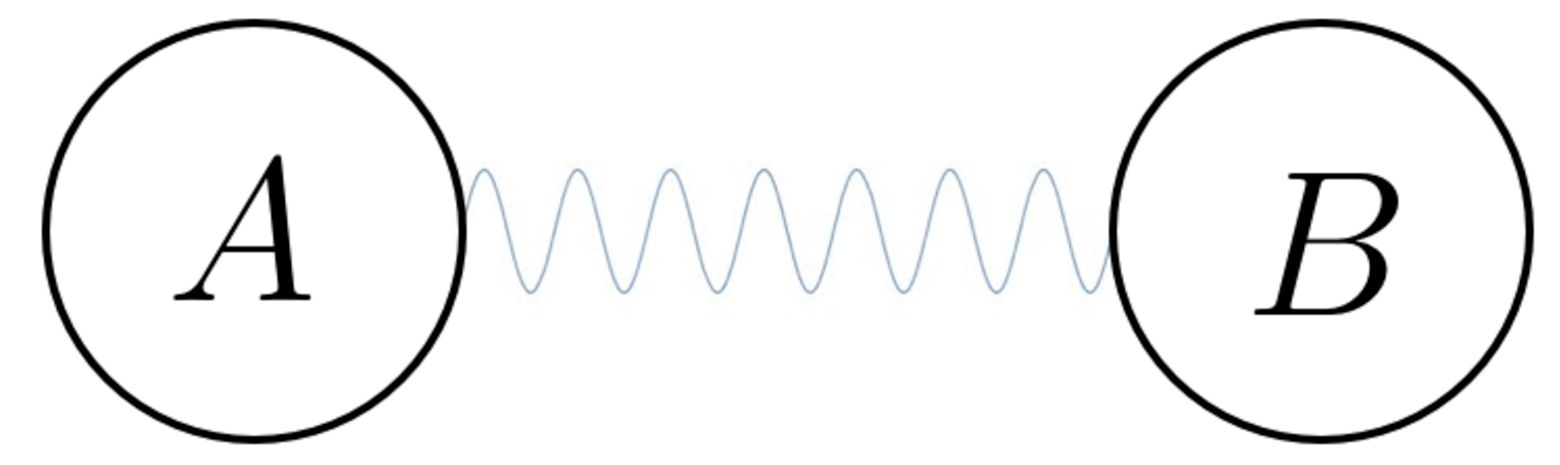
\includegraphics[width =0.49\textwidth]{subsystems.pdf}
\caption{Two quantum systems, $A$ and $B$ coupled such that the quantum state of the complete system lives in a Hilbert space that is the tensor product of the Hilbert spaces of $A$ and $B$.}
\label{fig:coupledSubsystems}
\end{center}
\end{figure}

\noindent In the Schmidt basis\cite{Knight1994} a quantum state, $\ket{\psi}$, of system $C$ can be expressed in terms of the basis vectors of systems $A$ and $B$,
\begin{equation}
\ket{\psi} = \sum_{n}\alpha_{n}\ket{a_n}\otimes\ket{b_n}.
\end{equation}
With $\ket{a_n}\in\mathcal{H}_A$ and $\ket{b_n}\in\mathcal{H}_B$. Now consider taking a measurement, $O_A$, on system $A$ without touching $B$, the expected outcome of this measurement is then,
\begin{eqnarray}
\bra{\psi}O_A \otimes \mathbb{1}_B\ket{\psi} &=& \bra{\psi} \sum_{n}\alpha_n O_A\ket{a_n}\otimes\ket{b_n} \\ &=& \sum_{n,m}\alpha_m^*\alpha_n\bra{a_m} O_A \ket{a_n}\otimes\langle b_m | b_n\rangle
\\ &=& \sum_n \lvert\alpha\rvert^2\bra{a_n} O_A \ket{a_n} \\
&=& \textnormal{Tr}_A(\rho_A O_A),
\end{eqnarray}
where $\mathbb{1}_B$ is the identity operator acting on system $B$, $\rho_A$ is the reduced density operator\footnote{it satisfies the three properties in Sec.~\ref{sec:DensityMatrix}} for system $A$ and $\textnormal{Tr}_A$ is the partial trace over the basis of system $B$. The reduced density operator, $\rho_A$ may be obtained by ``tracing out'' system $B$ from the projector onto state $\ket{\psi}\in\mathcal{H}_C$ i.e.

\begin{eqnarray}
\rho_C &=& \ket{\psi}\bra{\psi} = \sum_{n,m}\alpha_n\alpha_m^*\ket{a_n}\bra{a_m}\otimes\ket{b_n}\bra{b_m}\\
\rho_A &=& \textnormal{Tr}_B(\rho_C) = \sum_{n,m}\alpha_n\alpha_m^*\ket{a_n}\bra{a_m}\otimes\textnormal{Tr}(\ket{b_n}\bra{b_m})\\
&=&\sum_n \lvert \alpha\rvert^2 \ket{a_n} \bra{a_n}.
\label{eq:traceOut}
\end{eqnarray}
So in DMQMC, it is also possible to stochastically sample the reduced density matrix for a subsystem of the total system under study. From this it is possible to calculate expectation values for measurement on that subsystem. Moreover, it allows for some interesting measures of quantum entanglement between the subsystems $A$ and $B$.
% ------------------------------------------------------------------------

\section{Von-Neumann Entropy}

The Von-Neumann Entropy is an extension of the Shannon entropy, from classical information theory into quantum information theory. In classical information theory, the Shannon entropy for a probability distribution $q_1,\dots, q_n$ is 
\begin{equation}
S_C(q_1,\dots,q_n)=\sum_i q_i \log_2 1/q_i.
\end{equation}
Similarly for a quantum state living in a finite $D$-dimensional Hilbert space, the Von-Neumann entropy is
\begin{equation}
\label{eq:VonNeumannEntropy}
S_Q(\bm{\rho}) = -\textnormal{Tr}(\bm{\rho}\log_2\bm{\rho}) = \sum_i p_i \log_2 1/p_i,
\end{equation}
where $p_i$ are the eigenvalues of $\bm{\rho}$. It describes the purity of the system. If one considers the density matrix in diagonal form, the eigenvalues $p_i$ represent the probability of the system being in some state $\ket{i}$ of the diagonal basis. Hence, for a pure state one eigenvalue is unity, whilst all the others are zero, giving a zero Von-Neumann entropy. However, for a maximally entangled mixed state, with equally likely probabilities of being in any of the states $\ket{i}$ in the diagonal basis, the Von-Neumman entropy is $\log_2{D}$. 

Therefore, if the Von-Neumann entropy is calculated for the reduced density matrix for system $A$, in Fig.~\ref{fig:coupledSubsystems}, it measures the amount of quantum entanglement between systems $A$ and $B$. For example, if the Von-Neumann entropy is zero, then $A$ is a pure state and so there is no entanglement between $A$ and $B$, assuming that the overall system $C$ is in a pure state. On the other hand if the Von-Neumann entropy is $\log_2{D}$, then subsystem $A$ is in a fully mixed state and $A$ and $B$ must be maximally entangled.

In order to compute the Von-Neumann entropy (Eq.~\ref{eq:VonNeumannEntropy}), the subsystem $A$ must be sufficiently small so that the reduced density matrix can be diagonalised directly. The Von-Neumann entropy has not been properly tested due to time restrictions. 

% ------------------------------------------------------------------------

\section{Concurrence and Entanglement of Formation}

In 2001, Hill and Wootters~\cite{Hill1997} introduced a new measure of entanglement for a two-qubit mixed state. For the case where the total system is mixed, the Von-Neumann entropy is no longer a good measure of quantum entanglement, because both subsystems $A$ and $B$ can have non-zero entropy even if there is no entanglement. The measure, known as the ``entanglement of formation'' is a generalisation of Von-Neumann entropy. The entanglement of formation of a bipartite quantum system can be defined as ``the minimum number of singlets needed to create an ensemble of pure states that represents a mixed state''~\cite{Wootters2001}. In this case a ``singlet'' refers to a state with zero total spin. 

Another definition of the Von-Neumann entropy, $E(\Phi)$, is the number of singlet pairs, required to required to create a copy of a pure state $\ket{\Phi}$\cite{Wootters2001}.The number of singlets required to create a copy of some mixed state that is expressed as an ensemble of pure states, $\rho = \sum_{j=1}^N p_j\ket{\Phi_j}\bra{\Phi_j}$, can be written
\begin{equation}
N_s = \sum_{j=1}^N p_jE(\Phi_j).
\end{equation}
This number depends on the particular ensemble so the minimum over all pure-state decompositions is taken in order to pick out the irreducible entanglement of the mixed system
\begin{equation}
E_f(\rho) = \min\left( \sum_{j}^N p_jE(\Phi_j) \right).
\end{equation}

For the special case of a two-qubit mixed state the entanglement of formation can be calculated from a quantity known as ``concurrence''. For a reduced density matrix, $\bm{\rho}_A$, where in this case $A$ refers to a subsystem of two qubits, the concurrence is defined as
\begin{equation}
\mathcal{C}(\bm{\rho}_A) \equiv \textnormal{max}(0, \gamma_1-\gamma_2-\gamma_3-\gamma_4),
\end{equation}
in which $\gamma_1 > \gamma_2 > \gamma_3 > \gamma_4$ are the eigenvalues of the matrix
\begin{equation}
\bm{R} = \sqrt{\sqrt{\bm{\rho}_A}\tilde{\bm{\rho}}_A\sqrt{\bm{\rho}_A}} \textnormal{\phantom{---}with\phantom{---}}  \tilde{\bm{\rho}}_A = (\sigma_y\otimes\sigma_y)\bm{\rho}_A^*(\sigma_y\otimes\sigma_y),
\end{equation}
where $\sigma_y$ is the Pauli spin matrix for the $y$-direction.

The concurrence, $\mathcal{C}$, ranges from zero to one and is monotonically related to the entanglement of formation~\cite{Hill1997}. In this way the concurrence can also be regarded as a measure of entanglement. The entanglement of formation for two qubits~\cite{Wootters2001} is given by,
\begin{equation}
\mathcal{E}(\mathcal{C}) = h\left( \frac{1+\sqrt{1-\mathcal{C}^2}}{2}\right)
\textnormal{\phantom{---}with\phantom{---}}
h(x) = -x\log_2 x - (1-x)\log_2 (1-x).
\end{equation}

The concurrence is easy to compute for the Heisenberg model. If it is assumed that the Hamiltonian is real (as is the case in the Heisenberg model) and therefore that the reduced density matrix is also real, the problem is reduced to finding the moduli of the eigenvalues of 
\begin{equation}
\label{eq:concurrenceMatrix}
\tilde{\bm{R}} = \bm{\rho}_A(\sigma_y\otimes\sigma_y).
\end{equation}
As $\tilde{\bm{R}}$ is only a $4\times4$ matrix it is trivial to compute the concurrence.
% ------------------------------------------------------------------------
\section{Implementation of the ground-state entanglement estimators}
Whilst it is possible to calculate finite-temperature estimators for both the Von-Neumann entropy and Concurrence, the current implementation can only handle such estimators for the ground-state. This is because   the current implementation is based on previous FCIQMC code which only allows simulations for a single $M_S$ subspace. In FCIQMC the ground-state always lies within a known $M_S$. For example, in a simulation for the antiferromagnetic Heisenberg model with zero applied magnetic field the ground-state is within the $M_S=0$ subspace. Unfortunately, there was not enough time during this MSci project to adapt the code so that simulations could run in all subspaces simultaneously, which would allow for finite-temperature estimators of entanglement.

In the current implementation the reduced density matrix, for a specified subsystem of spins, is averaged over all $\beta>\beta_{gs}$, where $\beta_{gs}$ is the critical $\beta$ beyond which the simulation enters the ground-state. This is to ensure that the reduced density matrix has the highest possible accuracy before computing the entanglement estimators.

In order to obtain the reduced density matrix at a particular $\beta > \beta_{gs}$ the subsystem $B$ is traced out as in Eq.~\ref{eq:traceOut}. This was achieved by looping over all elements of the total density matrix with non-zero psip populations and determining whether a particular element contributed towards the reduced density matrix. A simple test (see Fig.~\ref{fig:rdm_algorithm}) was devised to determine whether this was the case:

\begin{enumerate}
\item Define a boolean mask for subsystem $B$ - this is created at the start of the simulation and has bits set to 1 where a spin is to be included in subsystem $B$.
\item Perform a bit-wise \texttt{AND} operation on each of the two bit string ends that label the current density matrix element, with the boolean mask for subsystem $B$. This sets all bits that represent a spin in subsystem $A$ to 0 and leave those that represent a spin in $B$ unchanged.
\item If the two resultant bit strings are equal then this means that it lies on the diagonal of subsystem $B$ and hence contributes to the reduced density matrix for subsystem $A$. In this case, the psip charge on this element is added to the corresponding element of the reduced density matrix. If they are not equal then nothing is added to the reduced density matrix.
\end{enumerate}

\begin{figure}[H]
\begin{center}
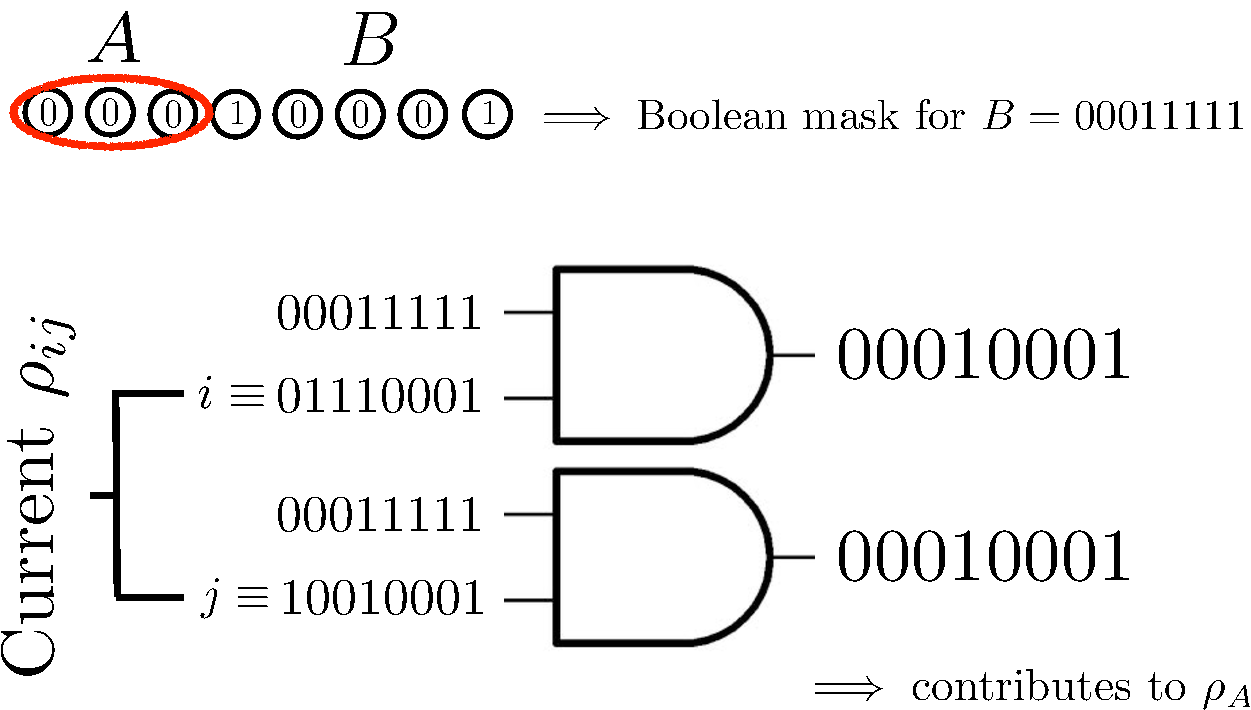
\includegraphics[width =0.8\textwidth]{rdm_algorithm.pdf}
\caption{Illustration of how a given density matrix element $\rho_{ij}$ is tested to see whether it contributes towards $\rho_A$ for the case that $A$ is 3 neighbouring spins on a chain of length $N=8$}
\label{fig:rdm_algorithm}
\end{center}
\end{figure}

After obtaining the average reduced density matrix, the Von-Neumann entropy is obtained by directly diagonalising the reduced density matrix\footnote{This is achieved using the \texttt{LAPACK ssyev} and \texttt{dsyev} routines for diagonalising symmetric matrices. These routines use the QR algorithm.}. For the concurrence, the matrix $\tilde{R}$ (Eq.~\ref{eq:concurrenceMatrix}) is diagonalised\footnote{This is achieved using the \texttt{LAPACK sgeev} and \texttt{dgeev} routines for diagonalising nonsymmetric matrices. Both routines first use Hessenberg reduction followed by the QR algorithm.}. This whole process is repeated over multiple $\beta$-loops to build up statistics and to enable the calculation of errors as in Sec.~\ref{sec:statErrCalc}.
% ------------------------------------------------------------------------
\section{Nearest-neighbour concurrence in Heisenberg rings}
The ground-state concurrence for neighbouring spins (qubits), illustrated in Fig.~\ref{fig:HeisenbergRing}, on a bipartite antiferromagnetic Heisenberg ring with $N$ qubits was first calculated by O'Connor and Wooters in 2001\cite{OConnor2001}. They found that the ground-state concurrence, $\mathcal{C}_{gs}$, is related to the ground-state energy, $E_{0}$, in the following way
\begin{equation}
\label{eq:groundstateConcurrence}
\mathcal{C}_{gs} = -\frac{1}{2}(E_{0}/N + 1).
\end{equation}

\begin{figure}[h!]
\begin{center}
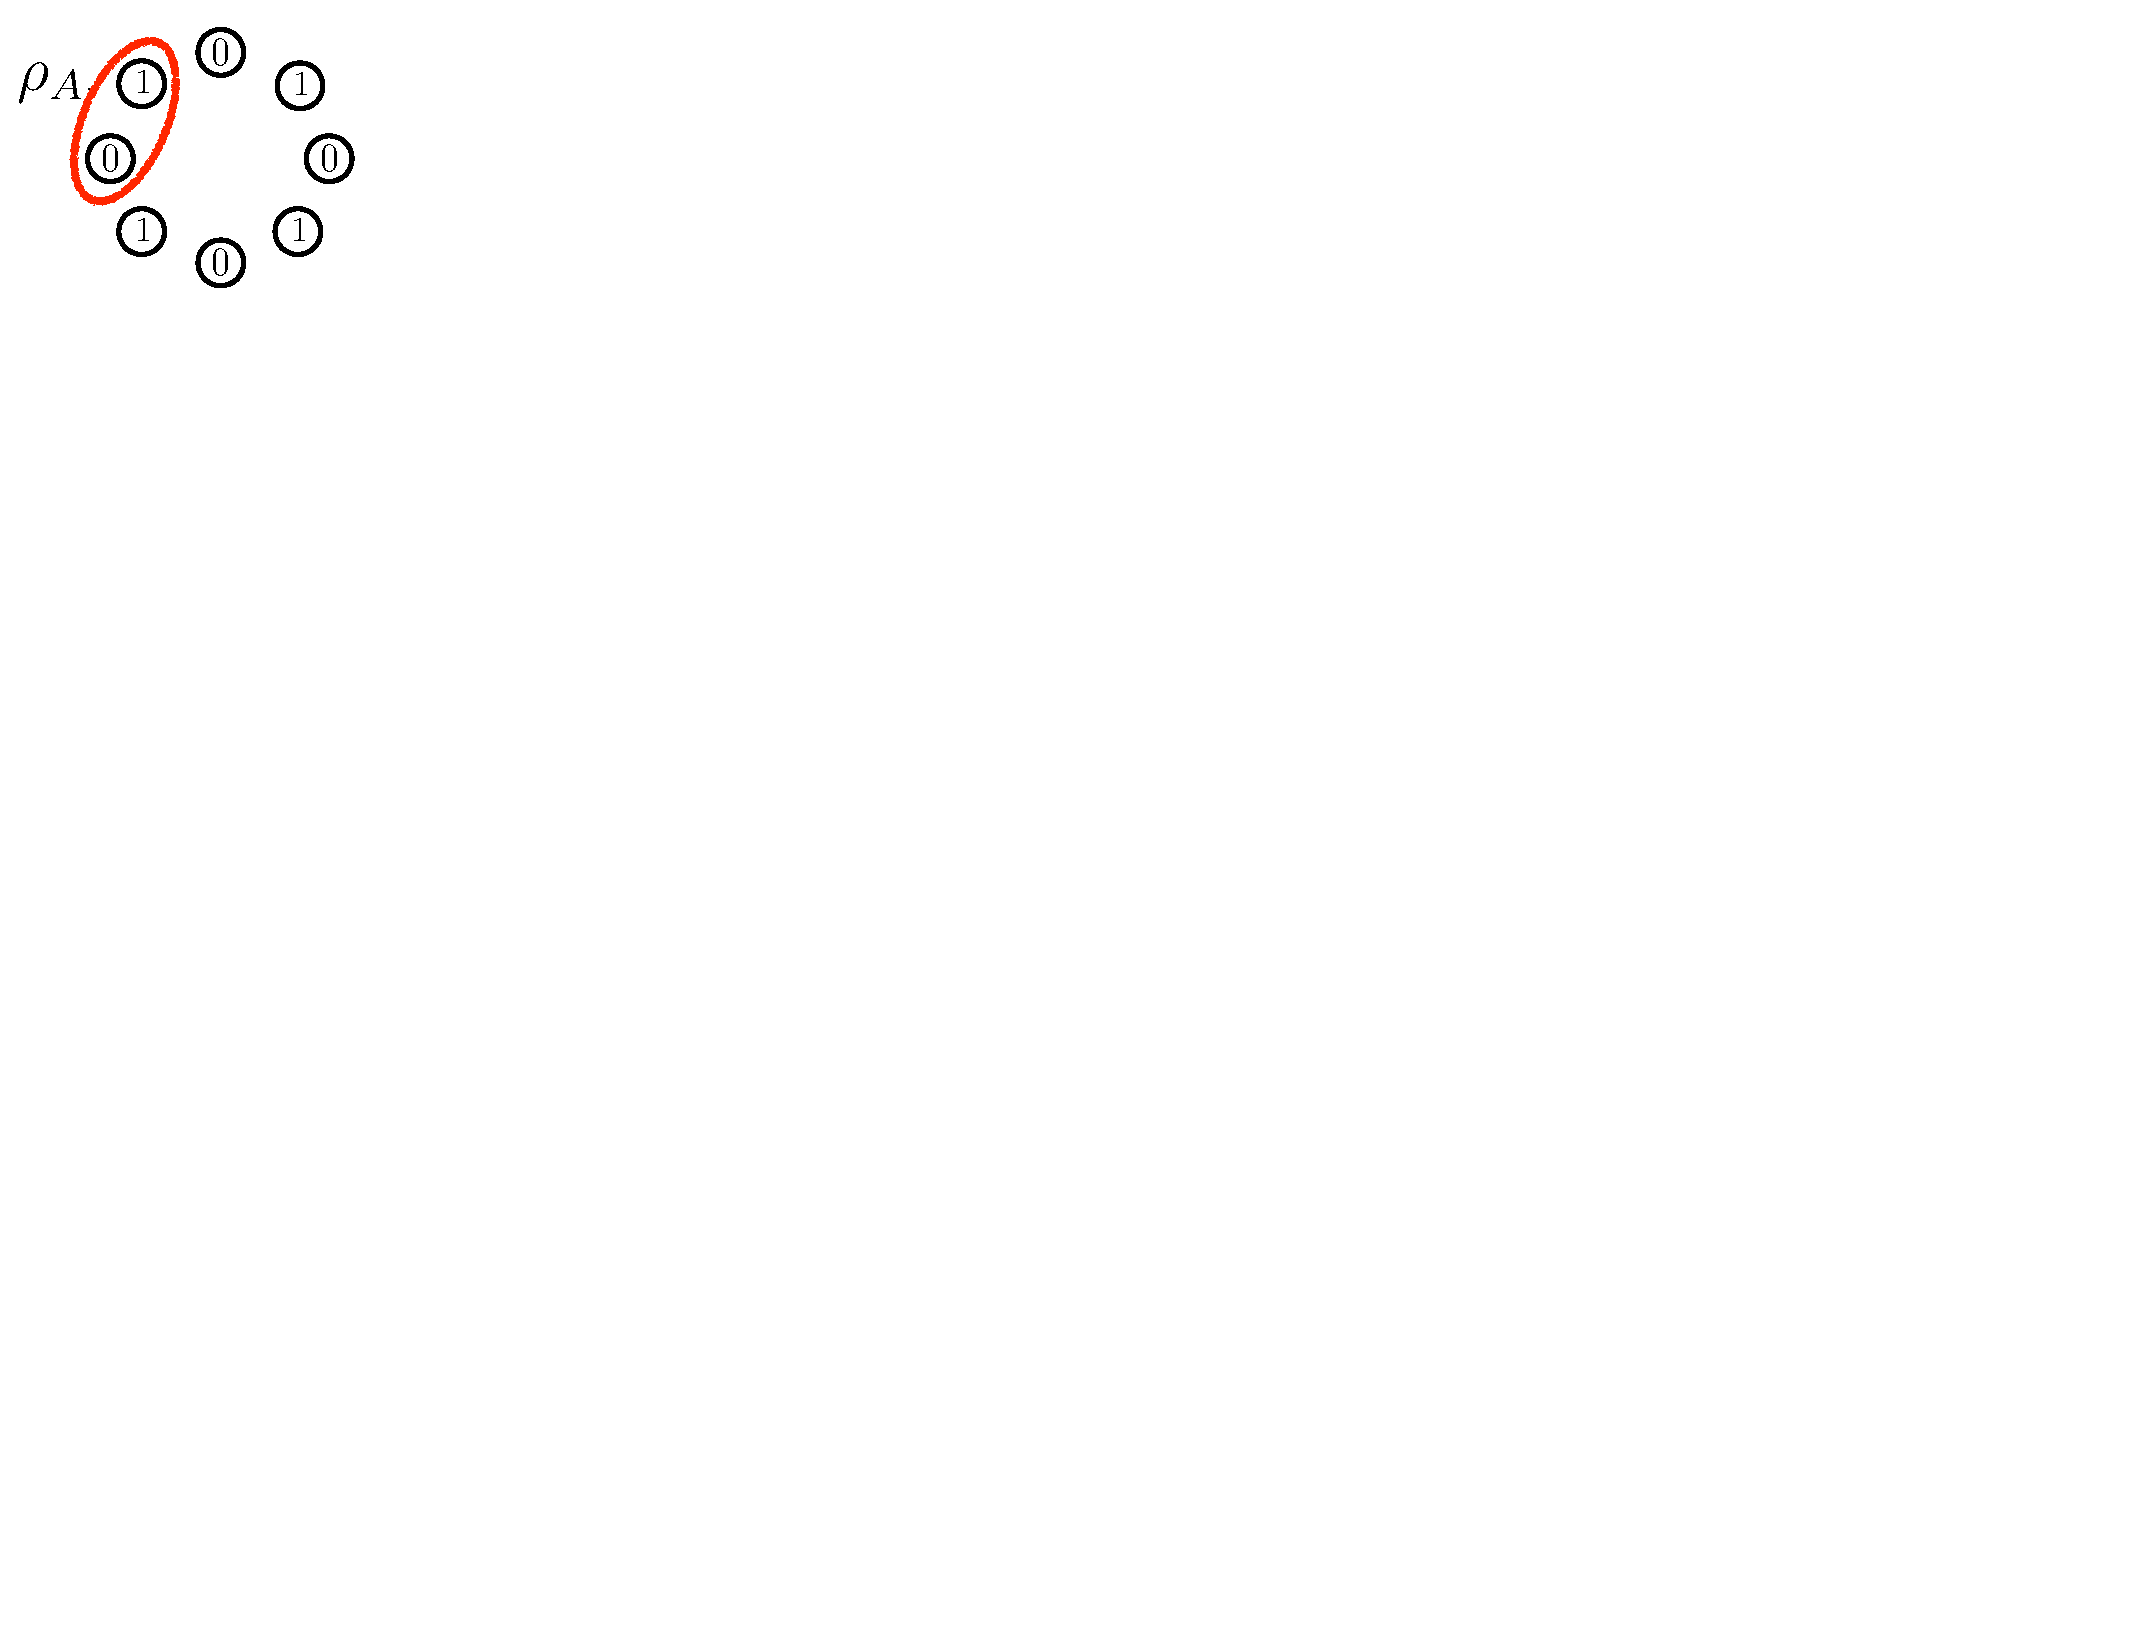
\includegraphics[width =0.49\textwidth]{HeisenbergRing.pdf}
\caption{Illustration of the subsystem of two qubits, $A$, on an $N = 8$ antiferromagnetic Heisenberg chain. The system can be regarded as a ring due to the periodic boundary conditions adopted.}
\label{fig:HeisenbergRing}
\end{center}
\end{figure}

To test whether the DMQMC ground-state concurrence estimator was implemented correctly, several Heisenberg rings of differing size were simulated. The results in Tab. 4.1, show that the DMQMC ground-state concurrence estimator was correct within error for bipartite rings up to $N=10$. Moreover, an $N=36$ Heisenberg ring was simulated with importance sampling and the ground-state concurrence of $\mathcal{C}_{gs} = 0.3873(8)$ was obtained. This agrees well with the value of $\mathcal{C}_{gs} = 0.38748(4)$ obtained from FCIQMC\cite{SpencerFCIQMC} and Eq.~\ref{eq:groundstateConcurrence}.
\begin{table}[H]
\begin{center}
{\scriptsize
\begin{tabular}{l | c c c c c c c c c}
$N$ & 2 & 4 & 6 & 8 & 10 & $\dots$ & 36 & $\infty$ \\ \hline
\cite{OConnor2001}$\mathcal{C}_{gs}$ & 1.000 & 0.500 & 0.434 & 0.412 & 0.403& $\dots$ & --& 0.386\\
DMQMC & 1.0006(6) & 0.5005(4) & 0.4342(5) & 0.4129(5) & 0.4031(4)& $\dots$ & 0.3873(8)& --
\end{tabular}
}
\caption{Comparision of the DMQMC ground-state concurrence calculation with the exact values for neighbouring qubits on a simple one dimensional bipartite antiferromagnetic Heisenberg ring of $N$ qubits.}
\end{center}
\label{tab:concHeisRing}
\end{table}

\section{Concurrence in a uniform magnetic field}
Applying a magnetic field to a system of spins changes the structure of the ground-state spin configuration and hence the ground-state entanglement properties of the system. In quantum information it is interesting to look at how the entanglement between qubits changes with a uniformly applied magnetic field. Since the magnetic field can be controlled it is possible to also control the amount of entanglement between certain qubits. %A QMC model that can calculate entanglement as a function of magnetic field could prove important in the development of quantum technologies.

As an example a uniform magnetic field was applied to a Heisenberg antiferromagnetic ring with $N=8$, the effect of which is shown in Fig.~\ref{fig:8_chain_concurrence_varying_mag_field}. Within a given $M_S$ subspace, changing the magnetic field shifts the diagonal elements of the Hamiltonian in Eq.~\ref{eq:MagneticHamiltonian}. Therefore, although the energy of the ground-state is changing, the ground-state wave function does not. Hence, for a given $M_S$ the concurrence between two neighbouring qubits does not change.
\begin{figure}[H]
\begin{center}
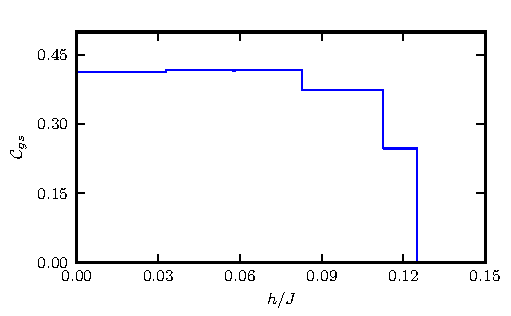
\includegraphics[width =1\textwidth]{8_chain_concurrence_varying_mag_field.pdf}
\caption{The ground-state concurrence, $\mathcal{C}_{gs}$, between two neighbouring qubits on an $N=8$ antiferromagnetic Heisenberg ring as a function of magnetic field strength in the ($z$-direction), $h$.}
\label{fig:8_chain_concurrence_varying_mag_field}
\end{center}
\end{figure}

However, when the lowest energy of a particular $M_S$ subspace is shifted so that it is higher than that of the next $M_S$, the ground-state wave function changes to one that belongs to the new $M_S$ subspace. As the form of the wave function changes so do the entanglement properties of the system. This explains, why in Fig.~\ref{fig:8_chain_concurrence_varying_mag_field} there are regions of constant entanglement. 

As the magnetic field increases, the amount of entanglement decreases as more spins are forced into alignment and the orientation of neighbouring spins becomes less correlated. Beyond a critical value of the magnetic field, $h/J = 0.125$, the concurrence drops to zero. This is the point where all spins become aligned and quantum correlations between neighbouring qubits disappears. It can be regarded as a quantum phase transition at $T=0$ due to quantum fluctuations, rather than thermal ones\cite{RudolphPrivate}.

\section{Concurrence with increasing separation}
Entanglement length\cite{Arnesen2001}, $l_E$, is another important property of many-body quantum systems that is relevant to quantum information theorists and experimentalists. It describes how quickly the entanglement between two qubits falls to zero as the separation between them is increased. 

In the Heisenberg model it is assumed that spin-spin interactions are short-range and between nearest neighbours. It is therefore difficult to find quantum correlations between spins that are not nearest neighbours. However, there is another critical value of the magnetic field, $h_{sym}$, for which an antiferromagnetic Heisenberg system is in the symmetric state
\begin{equation}
\psi_{sym} = \frac{1}{\sqrt{N}}(\ket{100\dots0} + \ket{010\dots0} + \ket{001\dots0} + \dots + \ket{000\dots1}).
\end{equation}
In this state it is evident that there is non-zero entanglement between any two qubits. This makes it possible to study how the entanglement between qubits changes as the distance between them is varied. Another benefit of this is that at this critical magnetic field the number of possible spin configurations is small and DMQMC can simulate the system very accurately.

Fig.~\ref{fig:concurrence36ChainSeparation} shows how the concurrence drops off as the distance between the two qubits increases, for an antiferromagnetic Heisenberg ring with $N=36$. Ignoring the effects near $d=0$ from the periodic boundary conditions, it can be seen that the concurrence approaches $\mathcal{C}_{gs} \propto e^{-d}$. Hence the entanglement length approaches $l_E \approx 1$. This makes sense as in the Heisenberg model it is approximated that the $J$-coupling occurs between nearest neighbours only and entanglement between non-nearest neighbours is due to non-direct interactions.
\begin{figure}[H]
\begin{center}
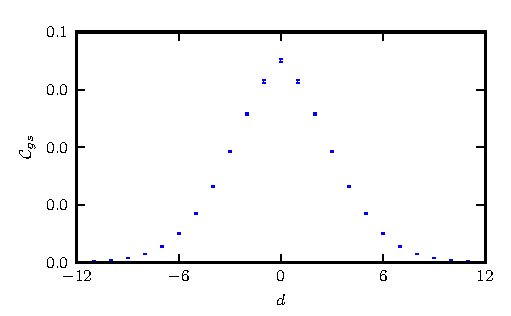
\includegraphics[width =1\textwidth]{36_chain_concurrence.pdf}\\
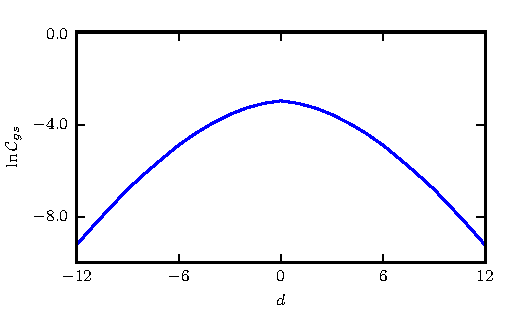
\includegraphics[width =1\textwidth]{36_log_chain_concurrence.pdf}
\caption[Ground-state concurrence with statistical errors (top) and logarithm of ground-state concurrence (bottom) for the $N=36$ antiferromagnetic Heisenberg ring, with $h/J  = 1.37$, as a function of separation between the two qubits.]{Ground-state concurrence with statistical errors (top) and logarithm of ground-state concurrence (bottom) for the $N=36$ antiferromagnetic Heisenberg ring, with $h/J  = 1.37$, as a function of separation between the two qubits. For example, $d=0$ is nearest neighbours, $d=1$ is next-nearest neighbours etc. It was difficult to obtain good statistics for $\lvert d\rvert > 10$ as the concurrence was so small. }
\label{fig:concurrence36ChainSeparation}
\end{center}
\end{figure}

\section{Summary}

In this chapter two quantum entanglement measures, the Von-Neumann entropy and the concurrence, were introduced. And the integration of these entanglement estimators into the DMQMC algorithm was discussed. The ground-state concurrence estimator was tested on one dimensional antiferromagnetic Heisenberg rings and the results were found to agree very well with the analytic values. 

Next the effects of a magnetic field on the entanglement between two nearest-neighbour qubits on an $N=8$ antiferromagnetic Heisenberg ring were studied.  It was found that there were quantum sharp transitions between different levels of entanglement due to quantum phase transitions. Finally, DMQMC was used to study how the entanglement between two qubits falls off as a function of the separation between them. It was found that there was a unit entanglement length, which agrees with the assumption in the Heisenberg model that interactions are only between nearest-neighbours.

%%% Local Variables: 
%%% mode: latex
%%% TeX-master: "../thesis"
%%% End: 
